\documentclass{ximera}

\input{../../../preamble.tex}


\definecolor{fvdnavy}{HTML}{071D43}
\definecolor{fvdcyan}{HTML}{20BFC6}
\definecolor{fvdcyanlight}{HTML}{EFFCFB}
\definecolor{fvdmagenta}{HTML}{F10D69}
\definecolor{fvdmagentalight}{HTML}{FFF1F7}
\definecolor{fvdtext}{HTML}{163044}





%=================================================
% Pedagogische omgevingen
% PDF: tcolorbox
% HTML: learning-box
%=================================================

\newenvironment{voorkennis}
{%
    \ifdefined\HCode
        \HCode{%
<section class="learning-box learning-box--prior">
<div class="learning-box__header">
<span class="learning-box__icon" aria-hidden="true"></span>
<span class="learning-box__title">Voorkennis</span>
</div>
<div class="learning-box__content">
        }%
        \begin{itemize}
    \else
       \begin{tcolorbox}[
    enhanced,
    breakable,
    colback=fvdcyanlight,
    colframe=fvdcyan,
    coltext=fvdtext,
    boxrule=0.5pt,
    leftrule=4pt,
    arc=4mm,
    outer arc=4mm,
    left=7mm,
    right=6mm,
    top=5mm,
    bottom=5mm,
    before skip=6mm,
    after skip=6mm,
    title=Voorkennis,
    coltitle=fvdcyan,
    fonttitle=\bfseries\Large,
    attach title to upper={\par\smallskip},
    boxed title style={
        empty,
        left=0mm,
        right=0mm,
        top=0mm,
        bottom=0mm
    },
    overlay={
        \draw[
            fvdcyan,
            line width=0.5pt
        ]
        ([xshift=42mm,yshift=-13mm]frame.north west)
        --
        ([xshift=-7mm,yshift=-13mm]frame.north east);
    }
]
        \begin{itemize}
    \fi
}
{%
    \end{itemize}
    \ifdefined\HCode
        \HCode{%
</div>
</section>
        }%
    \else
        \end{tcolorbox}
    \fi
}


\newenvironment{leerdoelen}
{%
    \ifdefined\HCode
        \HCode{%
<section class="learning-box learning-box--goals">
<div class="learning-box__header">
<span class="learning-box__icon" aria-hidden="true"></span>
<span class="learning-box__title">Leerdoelen</span>
</div>
<div class="learning-box__content">
        }%
        \begin{itemize}
    \else
\begin{tcolorbox}[
    enhanced,
    breakable,
    colback=fvdmagentalight,
    colframe=fvdmagenta,
    coltext=fvdtext,
    boxrule=0.5pt,
    leftrule=4pt,
    arc=4mm,
    outer arc=4mm,
    left=7mm,
    right=6mm,
    top=5mm,
    bottom=5mm,
    before skip=6mm,
    after skip=6mm,
    title=Leerdoelen,
    coltitle=fvdmagenta,
    fonttitle=\bfseries\Large,
    attach title to upper={\par\smallskip},
    boxed title style={
        empty,
        left=0mm,
        right=0mm,
        top=0mm,
        bottom=0mm
    },
    overlay={
        \draw[
            fvdmagenta,
            line width=0.5pt
        ]
        ([xshift=42mm,yshift=-13mm]frame.north west)
        --
        ([xshift=-7mm,yshift=-13mm]frame.north east);
    }
]
        \begin{itemize}
    \fi
}
{%
    \end{itemize}
    \ifdefined\HCode
        \HCode{%
</div>
</section>
        }%
    \else
        \end{tcolorbox}
    \fi
}



\title{Stijgen, dalen en extrema}
\author{Ingmar Herreman}

\begin{document}

\fvdchapterdata{5}{Het gedrag van functies beschrijven}{2}

\begin{abstract}
Een grafiek laat zien hoe een functiewaarde verandert wanneer de invoer toeneemt.
We leren stijgende, dalende en constante intervallen herkennen, extrema correct
beschrijven en deze informatie verbinden met grafiek, tabel, voorschrift en context.
\end{abstract}

\maketitle

\begin{voorkennis}
Je kunt:
\begin{itemize}
  \item domein en bereik van een functie interpreteren;
  \item nulwaarden en tekenverloop uit een grafiek aflezen;
  \item functiewaarden vergelijken;
  \item intervallen correct noteren.
\end{itemize}
\end{voorkennis}

\begin{leerdoelen}
Na dit hoofdstuk kun je:
\begin{itemize}
  \item uit een grafiek bepalen waar een functie stijgt, daalt of constant is;
  \item stijgen en dalen formuleren door functiewaarden te vergelijken;
  \item lokale en globale maxima en minima herkennen en correct benoemen;
  \item onderscheid maken tussen een extremumplaats en een extremumwaarde;
  \item een verloopbeschrijving lezen en opstellen;
  \item vanuit gegeven kenmerken een mogelijke grafiek construeren;
  \item stijgen, dalen en extrema interpreteren in een betekenisvolle context;
  \item met GeoGebra kenmerken onderzoeken en vermoedens controleren.
\end{itemize}
\end{leerdoelen}

\FVDsection{Hoe verandert een functie?}

In het vorige hoofdstuk onderzochten we of functiewaarden positief, nul of negatief zijn.
Nu stellen we een andere vraag:

\[
\important{\text{Wat gebeurt er met }f(x)\text{ wanneer }x\text{ toeneemt?}}
\]

Denk aan de hoogte van een gelanceerd voorwerp, de temperatuur tijdens een experiment
of het elektrisch vermogen van een installatie. Een grootheid kan toenemen, afnemen
of gedurende een tijd onveranderd blijven.

\begin{center}
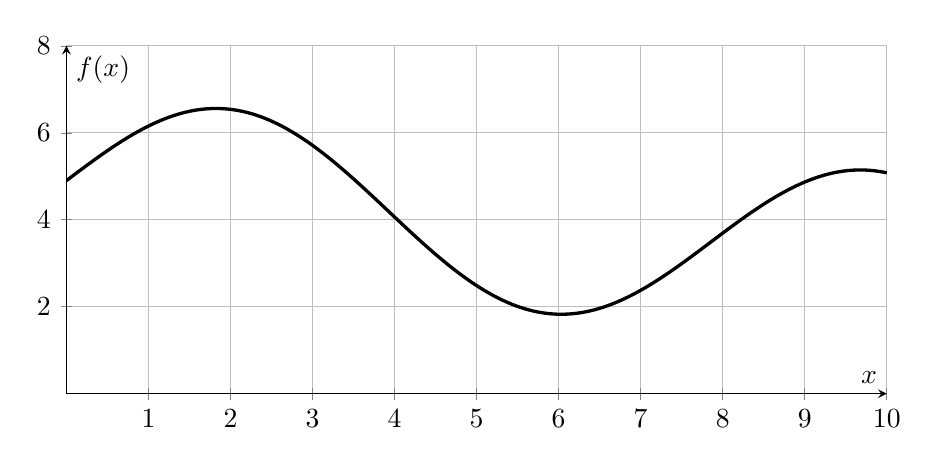
\begin{tikzpicture}
\begin{axis}[
  width=12cm,height=6cm,
  axis lines=middle,
  xmin=0,xmax=10,ymin=0,ymax=8,
  xlabel={$x$},ylabel={$f(x)$},
  grid=both,samples=200
]
\addplot[very thick,domain=0:10] {4+2*sin(deg(0.8*x))-0.18*(x-5)};
\end{axis}
\end{tikzpicture}
\end{center}

Bij het lezen van zo'n grafiek bewegen we steeds \textbf{van links naar rechts}.
We volgen dus toenemende \(x\)-waarden.

\FVDsection{Stijgend, dalend en constant}

\begin{definitie}
Een functie \(f\) is op een interval \(I\) \textbf{stijgend} als voor
\(x_1,x_2\in I\) met \(x_1<x_2\) geldt:
\[
f(x_1)\leq f(x_2).
\]

Ze is op \(I\) \textbf{dalend} als:
\[
x_1<x_2 \Longrightarrow f(x_1)\geq f(x_2).
\]

Ze is op \(I\) \textbf{constant} als:
\[
f(x_1)=f(x_2)
\]
voor alle \(x_1,x_2\in I\).
\end{definitie}

Grafisch betekent dit:
\[
\begin{array}{ccl}
\text{stijgend} &:& \text{de grafiek gaat van links naar rechts omhoog},\\
\text{dalend}   &:& \text{de grafiek gaat van links naar rechts omlaag},\\
\text{constant} &:& \text{de grafiek verloopt horizontaal}.
\end{array}
\]

\begin{opmerking}
``Stijgend'' betekent niet hetzelfde als ``positief''.
Een grafiek kan volledig onder de \(x\)-as liggen en toch stijgen.
Ook kan een positieve functie dalen.
Het \textbf{teken} beschrijft waar de grafiek ligt ten opzichte van de \(x\)-as;
het \textbf{verloop} beschrijft hoe de functiewaarden veranderen wanneer \(x\) toeneemt.
\end{opmerking}

\begin{voorbeeld}[Positief maar dalend]
Voor
\[
f(x)=\frac{1}{x},\qquad x>0,
\]
zijn alle functiewaarden positief. Toch wordt \(f(x)\) kleiner als \(x\) groter wordt.
De functie is dus dalend op \(]0,+\infty[\).
\end{voorbeeld}

\FVDsection{Van grafiek naar verloop}

Beschouw een functie met onderstaande grafiek.

\begin{center}
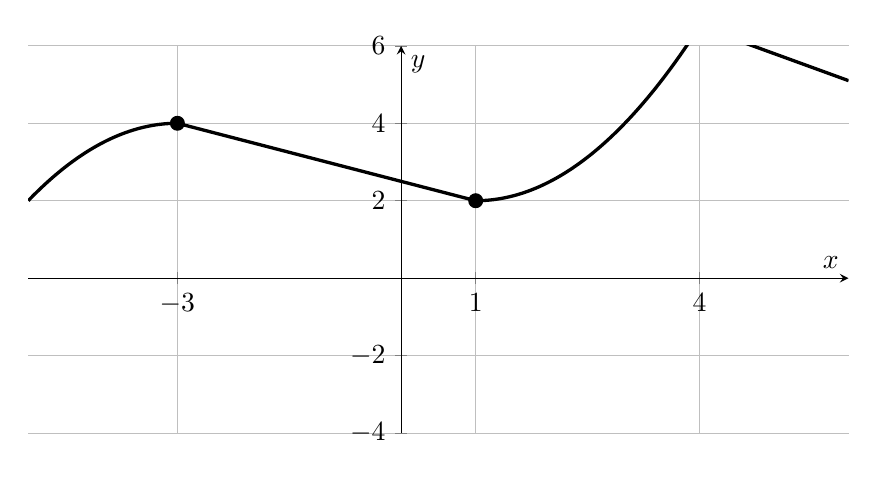
\begin{tikzpicture}
\begin{axis}[
  width=12cm,height=6.5cm,
  axis lines=middle,
  xmin=-5,xmax=6,ymin=-4,ymax=6,
  xlabel={$x$},ylabel={$y$},
  grid=both,
  xtick={-3,1,4},
  samples=200
]
\addplot[very thick,domain=-5:-3] {-0.5*(x+3)^2+4};
\addplot[very thick,domain=-3:1] {4-0.5*(x+3)};
\addplot[very thick,domain=1:4] {2+0.5*(x-1)^2};
\addplot[very thick,domain=4:6] {6.5-0.7*(x-4)};
\addplot[only marks,mark=*,mark size=2.5pt]
coordinates {(-3,4) (1,2) (4,6.5)};
\end{axis}
\end{tikzpicture}
\end{center}

We lezen van links naar rechts:
\begin{itemize}
  \item tot \(x=-3\) stijgt de functie;
  \item van \(x=-3\) tot \(x=1\) daalt ze;
  \item van \(x=1\) tot \(x=4\) stijgt ze opnieuw;
  \item na \(x=4\) daalt ze.
\end{itemize}

De punten waar het verloop van stijgend naar dalend of omgekeerd verandert,
zijn bijzondere punten. Daar ontstaan extrema.

\FVDsection{Maxima en minima}

\begin{definitie}
Een functie \(f\) heeft in \(x=a\) een \textbf{lokaal maximum}
als \(f(a)\) groter dan of gelijk is aan de functiewaarden in de onmiddellijke
omgeving van \(a\).

Een functie \(f\) heeft in \(x=a\) een \textbf{lokaal minimum}
als \(f(a)\) kleiner dan of gelijk is aan de functiewaarden in de onmiddellijke
omgeving van \(a\).
\end{definitie}

Een maximum of minimum noemen we een \textbf{extremum}.

\begin{eigenschap}[Verandering van verloop]
Grafisch herkennen we vaak:
\[
\text{stijgend}\longrightarrow\text{dalend}
\quad\Rightarrow\quad
\text{lokaal maximum},
\]
\[
\text{dalend}\longrightarrow\text{stijgend}
\quad\Rightarrow\quad
\text{lokaal minimum}.
\]
\end{eigenschap}

\begin{opmerking}[Plaats, waarde en punt]
Als \(f\) in \(x=a\) een maximum heeft, onderscheiden we:
\[
\text{extremumplaats}=a,\qquad
\text{extremumwaarde}=f(a),\qquad
\text{extremumpunt}=(a,f(a)).
\]
Deze drie begrippen zijn niet hetzelfde.
\end{opmerking}

\FVDsection{Lokaal en globaal}

Een lokaal extremum vergelijkt een functiewaarde met waarden \emph{in de buurt}.
Een globaal extremum vergelijkt met \emph{alle} functiewaarden op het beschouwde domein.

\begin{definitie}
\(f(a)\) is een \textbf{globaal maximum} als
\[
f(x)\leq f(a)
\]
voor elke \(x\) uit het domein.

\(f(a)\) is een \textbf{globaal minimum} als
\[
f(x)\geq f(a)
\]
voor elke \(x\) uit het domein.
\end{definitie}

\begin{opmerking}
Een lokaal maximum hoeft dus niet de grootste functiewaarde van de volledige functie te zijn.
Ook de keuze van het domein of het onderzochte interval kan bepalen of een extremum globaal is.
\end{opmerking}

\FVDsection{Een verlooptabel}

Net zoals een tekentabel het tekenverloop samenvat, kunnen we het stijgen en dalen
compact weergeven.

Stel dat een functie stijgt tot \(x=-2\), vervolgens daalt tot \(x=3\)
en daarna opnieuw stijgt. Dan kunnen we schrijven:

\[
\begin{array}{c|ccccc}
x & -\infty & & -2 & & 3 & & +\infty\\
\hline
f & & \nearrow & \text{max.} & \searrow & \text{min.} & \nearrow &
\end{array}
\]

De pijlen geven het verloop aan. De extrema liggen waar het verloop verandert.

\begin{opmerking}
Een verlooptabel bevat andere informatie dan een tekentabel.
Een tekentabel beschrijft het teken van \(f(x)\);
een verlooptabel beschrijft hoe \(f(x)\) verandert.
\end{opmerking}

\FVDsection{Van kenmerken terug naar een grafiek}

Analyseren betekent ook in de omgekeerde richting kunnen redeneren.

Stel dat we weten:
\[
\begin{array}{c|ccccccc}
x & -\infty && -2 && 1 && +\infty\\
\hline
f & &\nearrow& 4 &\searrow& -1 &\nearrow&
\end{array}
\]

Dan weten we onder meer:
\begin{itemize}
  \item \((-2,4)\) is een lokaal maximumpunt;
  \item \((1,-1)\) is een lokaal minimumpunt;
  \item links van \(-2\) stijgt de grafiek;
  \item tussen \(-2\) en \(1\) daalt ze;
  \item rechts van \(1\) stijgt ze.
\end{itemize}

Er bestaan nog steeds meerdere grafieken die aan deze informatie voldoen.
Een verlooptabel bepaalt dus niet de volledige functie, maar legt wel belangrijke
kenmerken vast.

\FVDsection{Context: hoogte van een drone}

De hoogte \(h(t)\) van een drone wordt gedurende een testvlucht gemeten.

\begin{center}
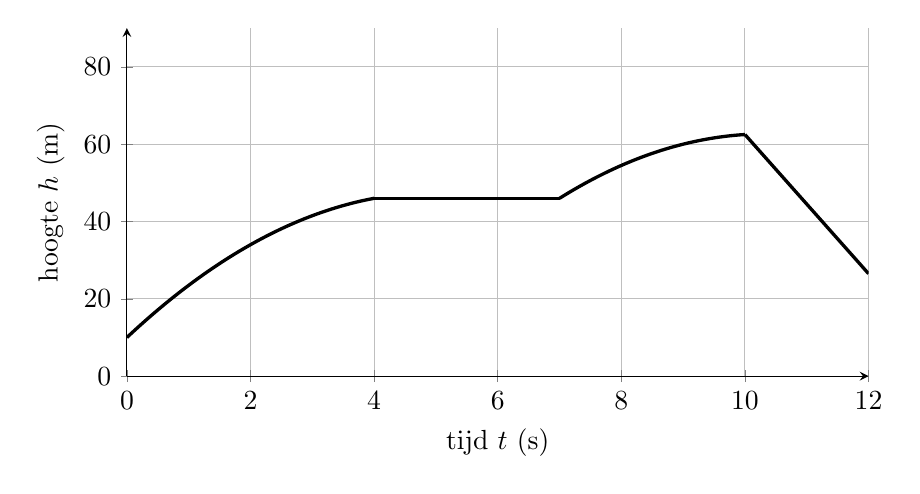
\begin{tikzpicture}
\begin{axis}[
  width=11cm,height=6cm,
  axis lines=left,
  xmin=0,xmax=12,ymin=0,ymax=90,
  xlabel={tijd \(t\) (s)},ylabel={hoogte \(h\) (m)},
  grid=both,
  samples=200
]
\addplot[very thick,domain=0:4] {10+15*x-1.5*x^2};
\addplot[very thick,domain=4:7] {46};
\addplot[very thick,domain=7:10] {46+10*(x-7)-1.5*(x-7)^2};
\addplot[very thick,domain=10:12] {62.5-18*(x-10)};
\end{axis}
\end{tikzpicture}
\end{center}

Hier krijgt het verloop een concrete betekenis:
\begin{itemize}
  \item als \(h\) stijgt, wint de drone hoogte;
  \item als \(h\) constant is, blijft de hoogte gelijk;
  \item als \(h\) daalt, verliest de drone hoogte;
  \item een maximum van \(h\) stelt een grootste bereikte hoogte voor.
\end{itemize}

\begin{opmerking}[Demathematiseren]
``\(h\) is dalend'' is een wiskundige beschrijving.
In de context zeggen we bijvoorbeeld:
``de drone daalt'' of ``de hoogte van de drone neemt af''.
\end{opmerking}

\FVDsection{Onderzoeken met GeoGebra}

Voer in GeoGebra bijvoorbeeld in:
\[
f(x)=x^3-3x.
\]

Onderzoek de grafiek en:
\begin{enumerate}
  \item voorspel waar \(f\) stijgt en daalt;
  \item zoek grafisch de extrema;
  \item verplaats een punt \(A=(a,f(a))\) over de grafiek en vergelijk
        functiewaarden links en rechts van een vermoed extremum;
  \item controleer je intervallen;
  \item verander het voorschrift in \(g(x)=x^3-3x+4\).
        Welke verloopkenmerken veranderen en welke blijven behouden?
\end{enumerate}

\begin{opmerking}
In dit hoofdstuk gebruiken we nog geen afgeleiden om stijgen, dalen en extrema te bepalen.
We analyseren het gedrag rechtstreeks vanuit grafiek, functiewaarden en kenmerken.
Later zullen afgeleiden hiervoor een krachtig nieuw instrument leveren.
\end{opmerking}

\FVDsection{Samenvatting}

\[
\boxed{
\text{grafiek}
\longleftrightarrow
\text{stijgen/dalen/constant}
\longleftrightarrow
\text{extrema}
\longleftrightarrow
\text{verlooptabel}
\longleftrightarrow
\text{context}
}
\]

Onthoud:
\begin{itemize}
  \item lees verloop steeds van links naar rechts;
  \item stijgend/dalend gaat over verandering van functiewaarden, niet over hun teken;
  \item stijgend \(\to\) dalend wijst op een lokaal maximum;
  \item dalend \(\to\) stijgend wijst op een lokaal minimum;
  \item onderscheid extremumplaats, extremumwaarde en extremumpunt;
  \item lokaal en globaal zijn verschillende begrippen;
  \item een verlooptabel moet je ook terug naar grafische informatie kunnen vertalen.
\end{itemize}

\end{document}
